\chapter{Flood Fill and Connected Components}
\label{ch:lesson04}

Once we have a binary image (e.g., from thresholding, Chapter~\ref{ch:lesson03}), a natural next question is: \emph{how many separate blobs are there, and where are they?} Two tools answer this:
\begin{itemize}
  \item \textbf{Flood fill} grows a region from a single seed pixel, spreading to all connected neighbors that share a similar value.
  \item \textbf{Connected component labeling} finds \emph{all} such regions in a binary image at once, labeling each with a unique ID.
\end{itemize}
Figure~\ref{fig:l04-1} shows the test image used throughout this chapter.

\begin{figure}[h]
\centering
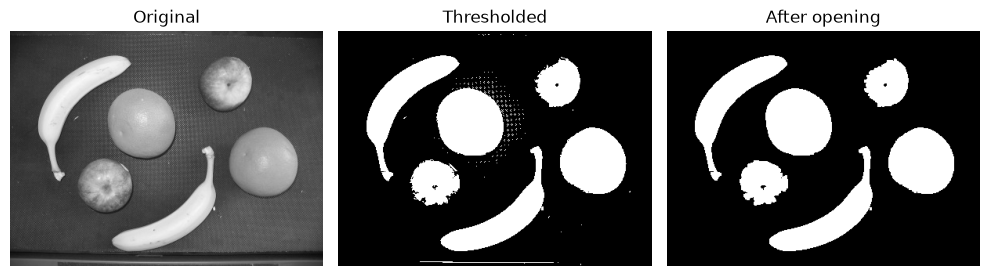
\includegraphics[width=0.95\textwidth]{figures/lesson04_fig01.png}
\caption{A photo of fruit, thresholded with Otsu's method (Chapter~\ref{ch:lesson03}), then cleaned up with a morphological opening. \attrib{Photo: Stan Birchfield.}}
\label{fig:l04-1}
\end{figure}

\section{Flood fill from a seed point}

Flood fill starts at a seed pixel and spreads outward to all connected pixels within a tolerance of the seed value, painting them a new color. The classic algorithm keeps a \emph{frontier} of pixels still to visit:

\begin{lstlisting}
def flood_fill_stack(binary, seed):
    filled = np.zeros_like(binary, dtype=bool)
    h, w = binary.shape
    stack = [seed]
    while stack:
        x, y = stack.pop()
        if x < 0 or x >= w or y < 0 or y >= h:
            continue
        if filled[y, x] or binary[y, x] == 0:
            continue
        filled[y, x] = True
        stack.extend([(x+1, y), (x-1, y), (x, y+1), (x, y-1)])
    return filled
\end{lstlisting}

\code{cv2.floodFill} does exactly the same thing, considerably faster because it is compiled. Figure~\ref{fig:l04-2} compares the two.

\begin{figure}[h]
\centering
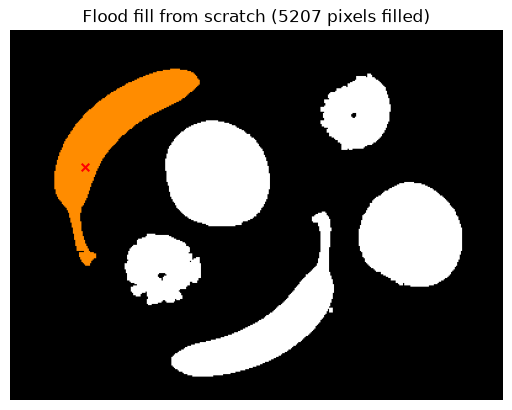
\includegraphics[width=0.46\textwidth]{figures/lesson04_fig02.png}\hspace{0.02\textwidth}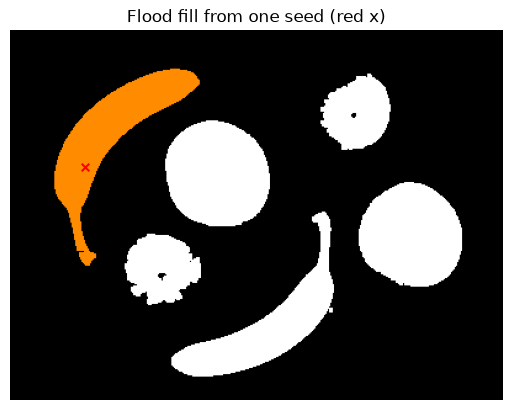
\includegraphics[width=0.46\textwidth]{figures/lesson04_fig03.png}
\caption{Flood fill from a single seed (red $\times$): the hand-written stack version (left) and \code{cv2.floodFill} (right) fill an identical region.}
\label{fig:l04-2}
\end{figure}

\section{Connected components: label every blob at once}

Instead of picking seeds by hand, connected-component labeling scans the whole image and assigns every blob its own integer label:

\begin{lstlisting}
num_labels, labels, stats, centroids = \
    cv2.connectedComponentsWithStats(im_bin, connectivity=8)
\end{lstlisting}

The classic algorithm --- omitted here for brevity --- is known as \emph{union-find}: two passes through the image, plus a traversal of an equivalence table. It also returns handy per-blob statistics (bounding box, area, centroid) essentially for free, since they require almost no extra computation (Chapter~\ref{ch:lesson05}). Figure~\ref{fig:l04-3} shows the labeled result.

\begin{figure}[h]
\centering
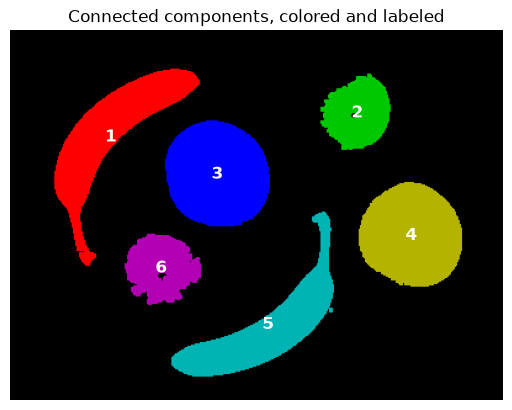
\includegraphics[width=0.55\textwidth]{figures/lesson04_fig04.png}
\caption{Each connected blob labeled with a distinct color and its integer ID.}
\label{fig:l04-3}
\end{figure}

\section{Filtering blobs by size}

A common use of connected components is to discard small, noise-like blobs and keep only significant ones, by thresholding on \code{stats[label, cv2.CC\_STAT\_AREA]}, as in Figure~\ref{fig:l04-4}.

\begin{figure}[h]
\centering
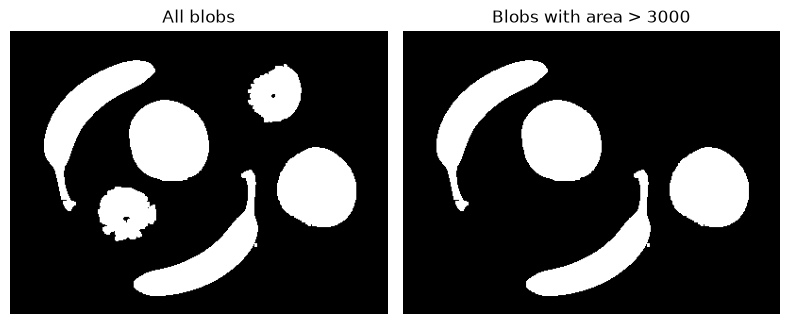
\includegraphics[width=0.75\textwidth]{figures/lesson04_fig05.png}
\caption{All blobs (left) versus only blobs with area above a chosen cutoff (right), which discards the two smallest apples.}
\label{fig:l04-4}
\end{figure}

\subsection*{Exercises}
\begin{enumerate}
  \item Change \code{connectivity=8} to \code{connectivity=4}. Construct a binary image (e.g., a diagonal staircase of single pixels) where 4-connectivity and 8-connectivity give a \emph{different} number of components.
  \item Use \code{cv2.floodFill} with a nonzero \code{loDiff}/\code{upDiff} tolerance on a grayscale (not binary) image, and describe what changes.
\end{enumerate}

\vfill
\fullcode{lesson04}{lesson04_floodfill_connected_components}
